\documentclass[11pt]{memoir}
\usepackage{outline} 

\usepackage{graphicx} 
\usepackage{listings} 
\usepackage{xcolor}
\usepackage[T1]{fontenc}
\usepackage[spanish]{babel}
\usepackage{float}
\usepackage{amsmath}
\usepackage{subcaption}
\usepackage{wrapfig}
\usepackage{hyperref}
\usepackage{cleveref}

\usepackage{fancyhdr}
\usepackage[ left=3cm,right=3cm,top=2cm,bottom=3cm]{geometry}

\pagestyle{fancy}
\setlength{\parindent}{4em}
\setlength{\parskip}{1em}

% Huérfanas y viudas
\widowpenalty100000
\clubpenalty100000

\headheight = 50pt
\textheight = 646pt
\headsep = 25pt
\fancyhead[R]{
	
\includegraphics[width=50pt]{img/Escudo}
}

\lstset{ 
    language=Matlab, % choose the language of the code
    numbers=left, % where to put the line-numbers
    frame=single,
    breaklines=true,
	 breakatwhitespace=false,
	%morecomment=[l]{%}
}


\title{

\includegraphics[width=1.75in]{./img/Escudo.PNG} \\
\vspace*{1in}
\Huge\textbf{Detección de baterías de coche} 


\includegraphics[width=\textwidth]{img/Clarios}}
\author{Daniel Puente Ramírez
		\vspace*{1.5in} \\
		Hardware de Aplicación Específica\\
		Grado en Ingeniería Informática\\
        \textbf{Universidad de Burgos}\\
        Burgos, España
       } \date{\today}
%--------------------Make usable space all of page
%\setlength{\oddsidemargin}{0in} \setlength{\evensidemargin}{0in}
%\setlength{\topmargin}{0in}     \setlength{\headsep}{-.25in}
%\setlength{\textwidth}{6.5in}   \setlength{\textheight}{8.5in}
%--------------------Indention
\setlength{\parindent}{1cm}

\begin{document}
%--------------------Title Page
\maketitle
\clearpage
\thispagestyle{empty}
\tableofcontents
\thispagestyle{empty}
\newpage


\section{Introducción}
\setcounter{page}{1}
Esta práctica se encuentra enmarcada dentro de la signatura \textit{Hardware de Aplicación Específica} del Grado en Ingeniería Informática, 4º curso, de la Universidad de Burgos.

En ella se plantea el problema de contar baterías de coche, ver Sección~\ref{sec:problema}. Para la resolución de la misma se desean poner en práctica, y con ello demostrar lo aprendido a lo largo de la asignatura, la gran mayoría de conceptos y técnicas utilizadas a lo largo de las prácticas.

\vspace{5cm}
\section{Agradecimientos}
Agradecer a Clarios Iberia S.L. la colaboración con la práctica, cediendo el material que se va a utilizar de forma desinteresada. 
\newpage
\section{Planteamiento del problema}\label{sec:problema}
El problema ante el que nos encontramos se encuentra dentro de la etapa final de fabricación de baterías para coches. Después de todo el proceso de producción, llenado, reposo, \textit{testing} y etiquetado, las baterías han de ser paletizadas para su transporte. Debido a las características de los equipos de trabajo, no se desea contar con un sistema de Inteligencia Artificial, sino que se desea realizar un procesamiento de imágenes en tiempo real. 

La empresa desea contabilizar el número de baterías que han sido finalizadas por turno, para ello desea instalar una serie de cámaras sobre las cintas transportadoras previas al robot de paletizado, de cada línea, ver Figura~\ref{fig:overview}.

\textbf{NOTA:} El planteamiento del problema es para despliegue del producto en un sistema de tiempo real. Por motivos obvios y coherentes se va a realizar sobre vídeos \textit{a mano} en 3 líneas diferentes de la planta de fabricación. 

Además, cada línea está organizada de manera diferente, por lo tanto, no todas cuentan con el mismo espacio vertical para colocar la cámara, el sistema deberá de ser capaz de detectar las baterías en un rango de entre veinticinco y cincuenta centímetros a la cinta de transporte.

\begin{figure}[H]
\centering

\begin{subfigure}{0.3\textwidth}
\centering
  \includegraphics[width = \textwidth, angle=270]{img/overview}
  \caption{Zona de paletizado}
  \label{fig:palet-zone}
\end{subfigure}\hfill
\begin{subfigure}{0.3\textwidth}
\centering
  \includegraphics[width = \textwidth, angle=90]{img/overview1}
  \caption{Una sola zona de paletizado}
  \label{fig:palet-one}
\end{subfigure}\hfill
\begin{subfigure}{0.3\textwidth}
\centering
  \includegraphics[width = \textwidth, angle=270]{img/lateral-lejos}
  \caption{Zona de implantación}
  \label{fig:implantacion}
\end{subfigure}

\bigskip

\begin{subfigure}{0.3\textwidth}
\centering
  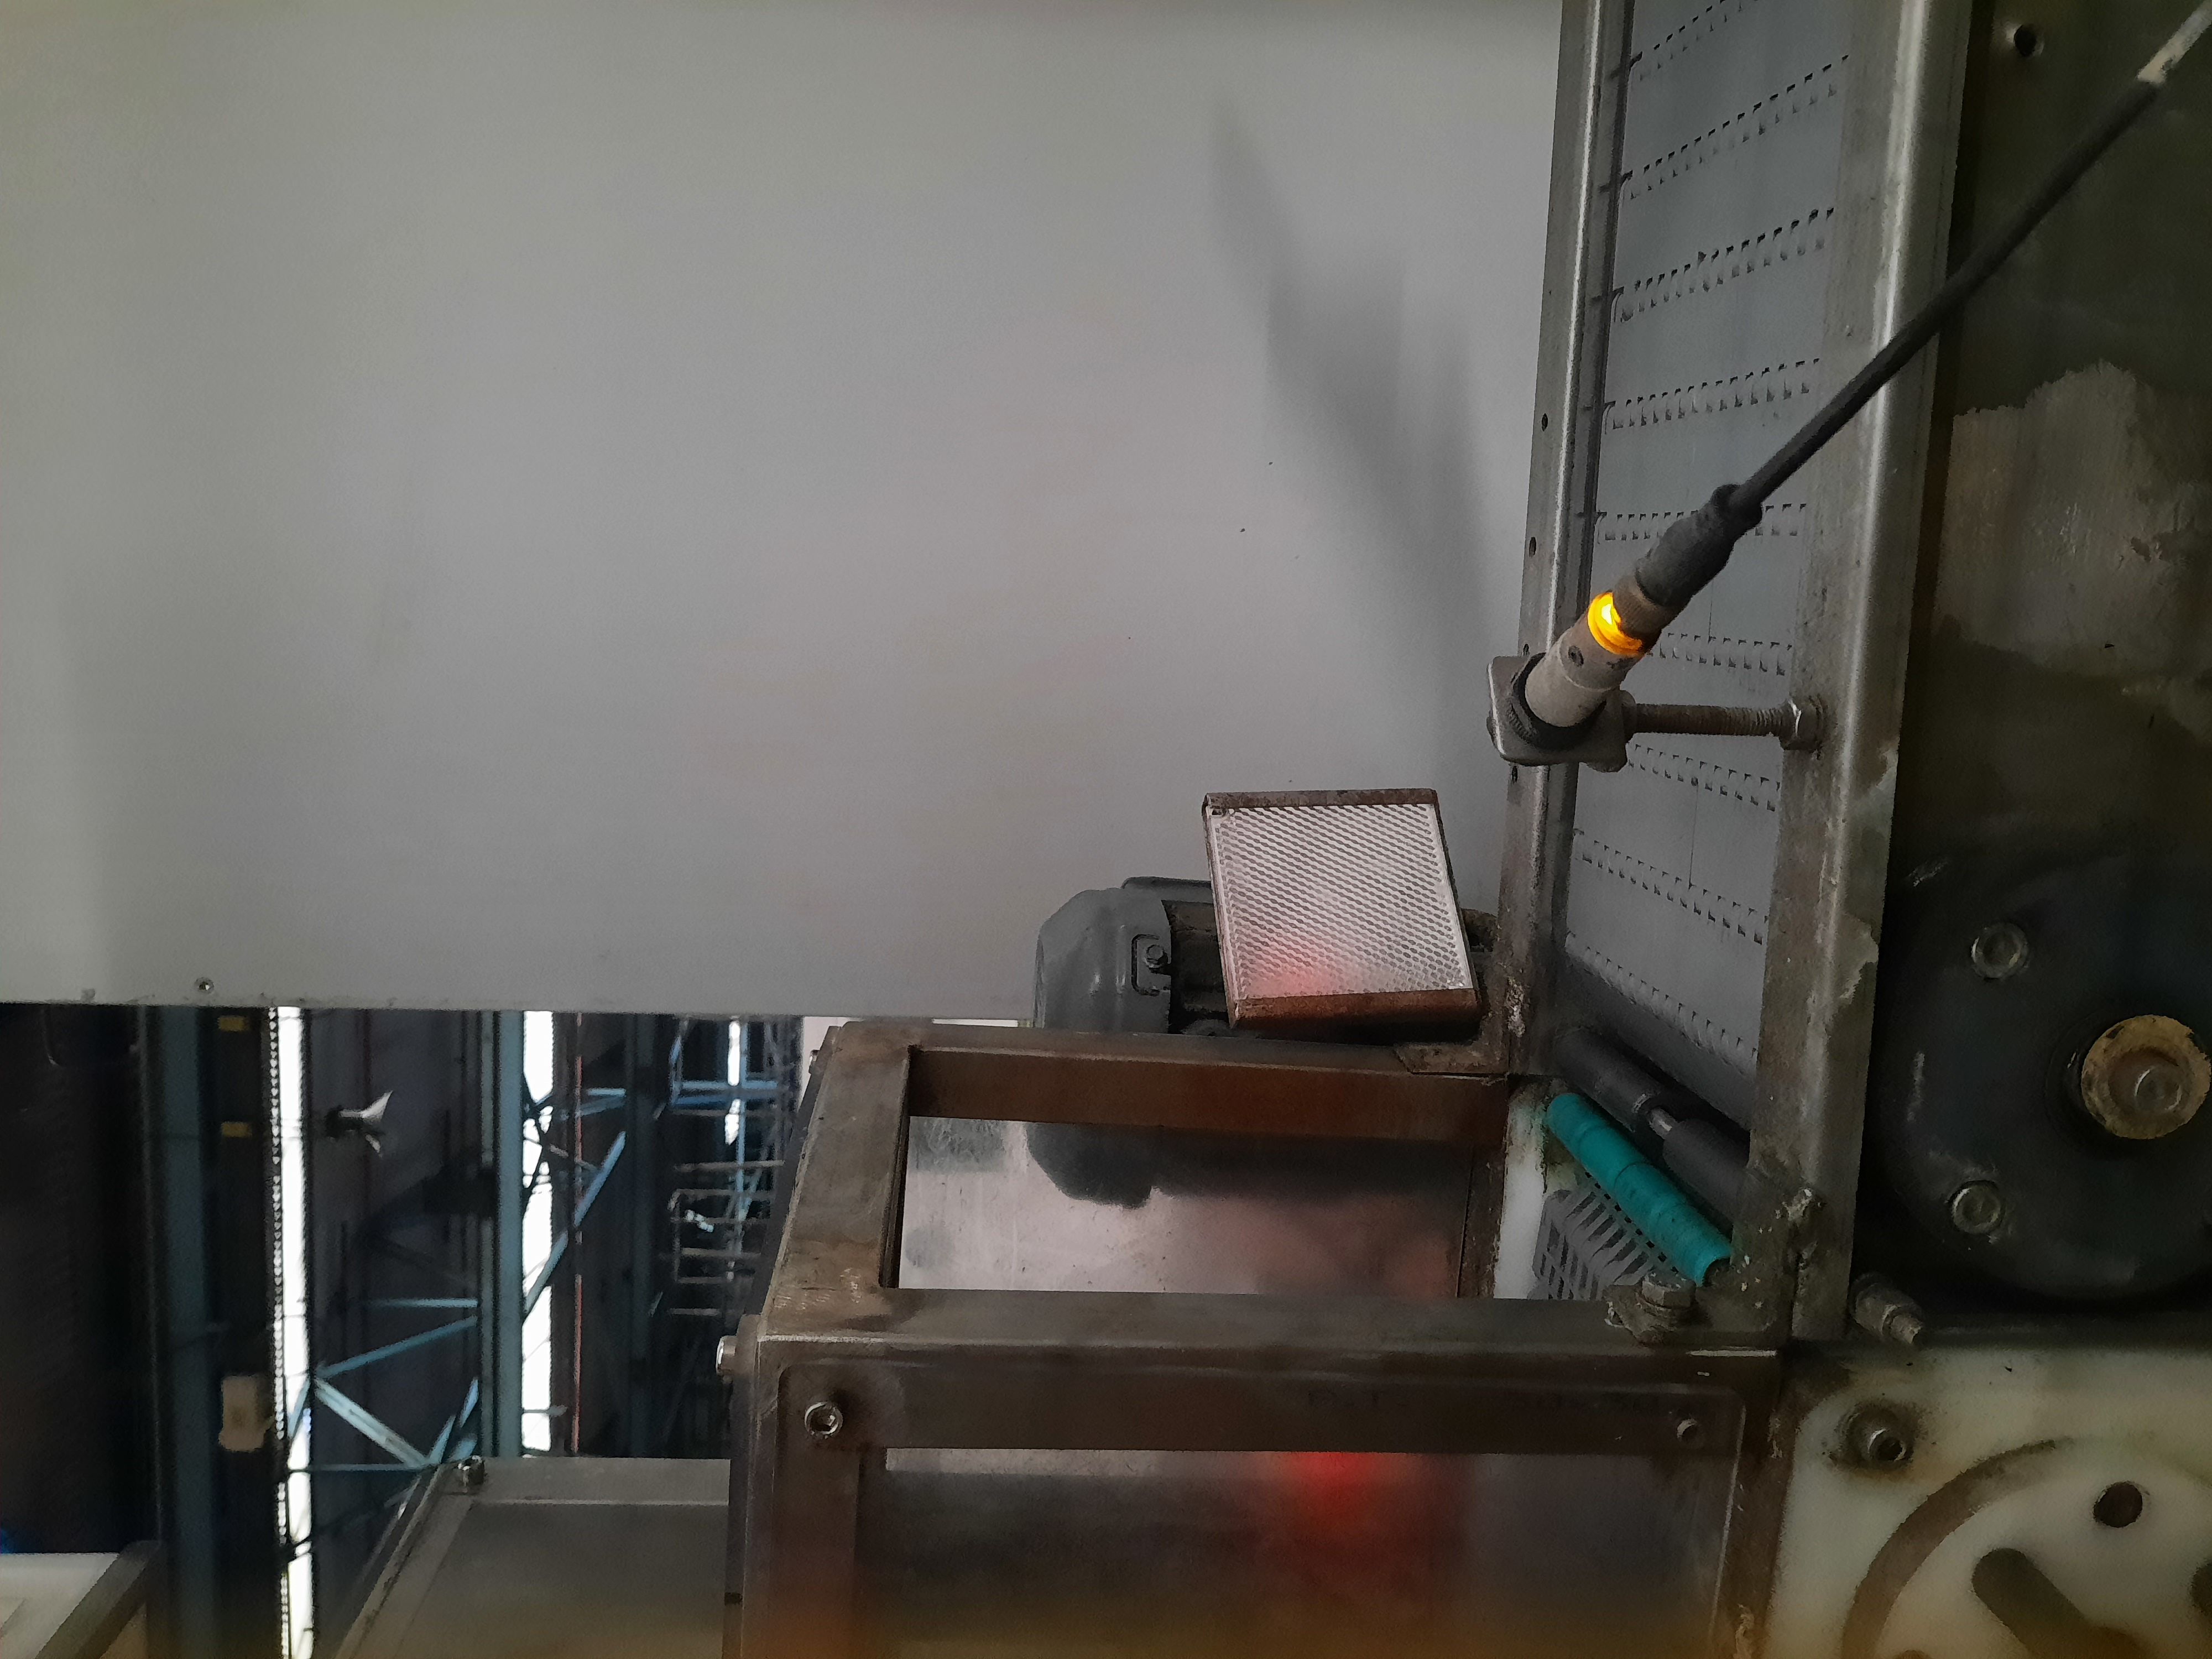
\includegraphics[width = \textwidth, angle=270]{img/closeup}
  \caption{Inicio cinta transporte}
  \label{fig:inicio}
\end{subfigure}\hfill
\begin{subfigure}{0.3\textwidth}
\centering
  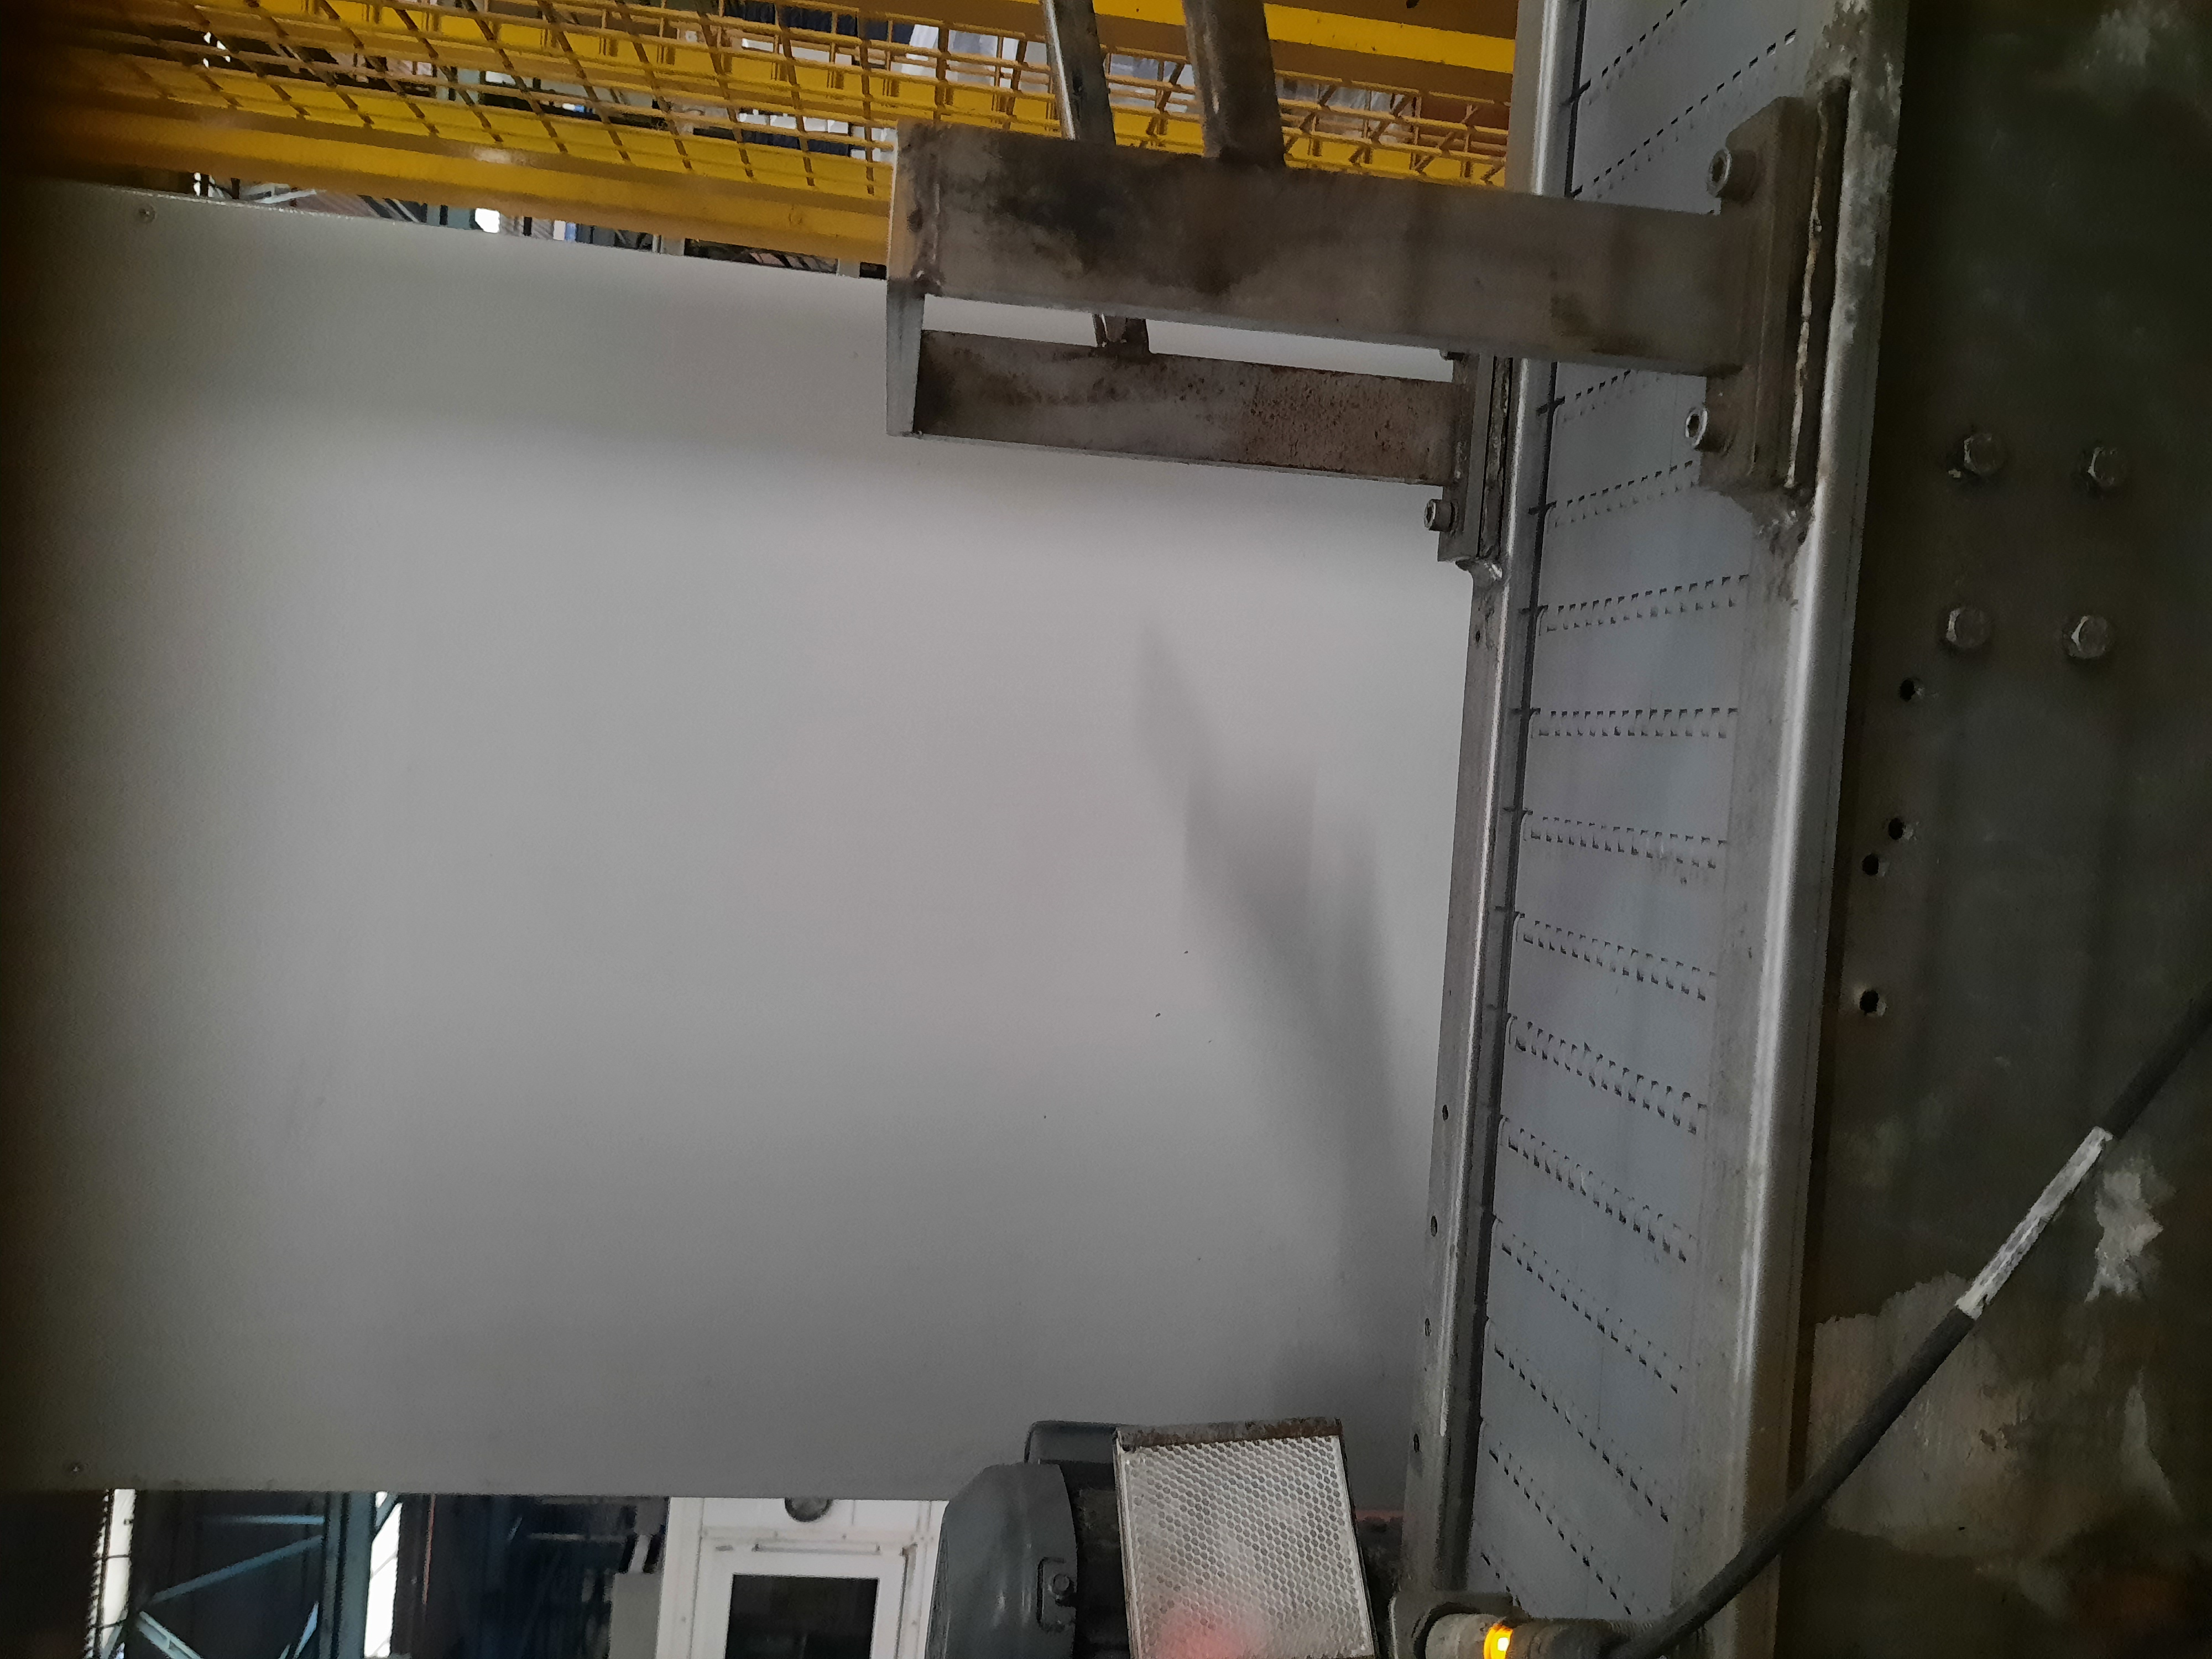
\includegraphics[width = \textwidth, angle=270]{img/closeup2}
  \caption{Entrada al robot}
  \label{fig:fin}
\end{subfigure}\hfill
\begin{subfigure}{0.3\textwidth}
\centering
  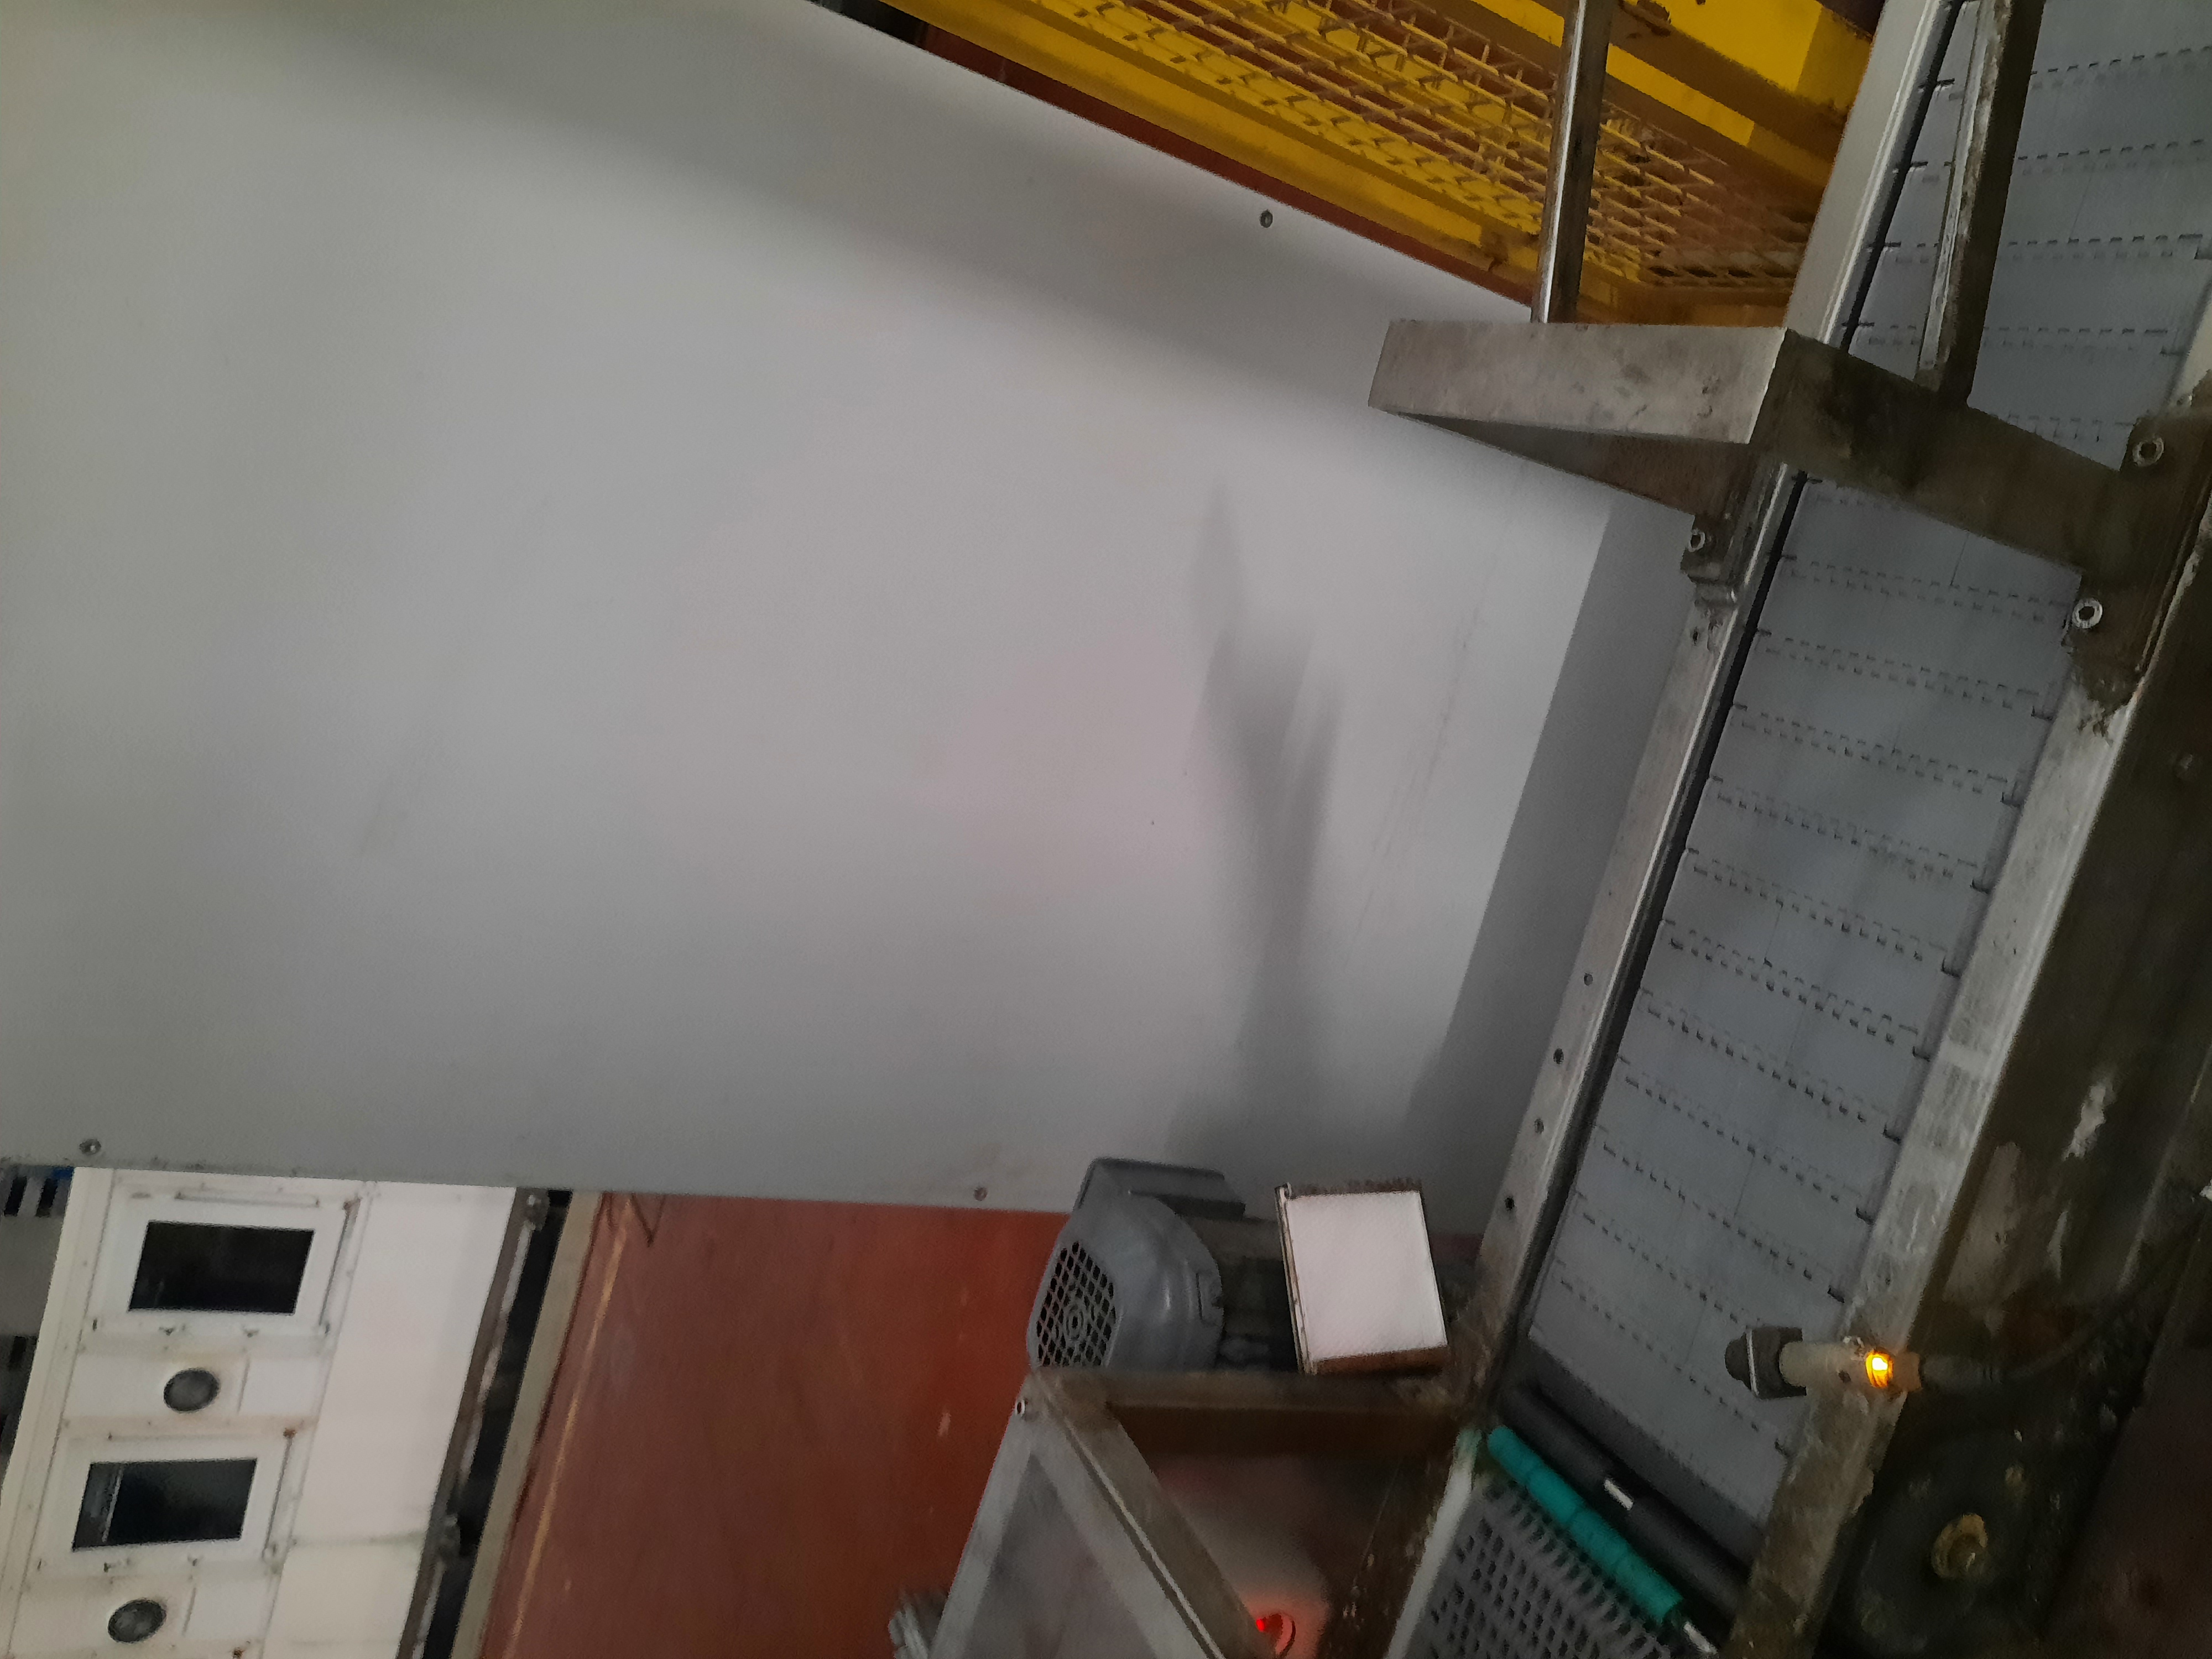
\includegraphics[width = \textwidth, angle=270]{img/angulo}
  \caption{Zona de detección}
  \label{fig:angulo}
\end{subfigure}

\caption{Vista de más a menos de la zona de trabajo}
\label{fig:overview}

\end{figure}

\newpage
\section{Resolución del problema}\label{sec:resolucion}
\subsection{Consideraciones importantes}
Antes de analizar la solución propuesta, debemos de tener en cuenta los siguientes apartados, ya que todos ellos influirán en mayor o menor medida en la codificación de la solución. \textbf{NOTA}. No se encuentran ordenadas de ninguna manera.
\begin{enumerate}
\item La distancia de la cámara a la cinta de transporte.
\item La distancia de la cámara a la batería.
\item El ángulo de la cámara con respecto a la cinta. Al encontrarse en una zona altamente robotizada y con muchas vibraciones, la cámara puede <<moverse>> con el paso del tiempo.
\item La cinta no está siempre en movimiento. Si el robot de paletizado se encuentra realizando la operación de carga, es decir, cogiendo baterías de la cinta, para evitar colisiones con las siguientes baterías, la cita se detiene. Por lo que una batería puede estar $n$ instantes temporales delante de la cámara.
\item El \textit{frame rate} de la cámara. 
\item El color de la batería.
\end{enumerate}

\subsection{Aproximación a la solución propuesta}
Con las consideraciones definidas, pasamos a la parte del análisis de las mismas y posterior planteamiento de la solución. Se van a comentar punto a punto, $[1-1, 2-2, \dots , n-n]$.

Una de las principales características que se desean es la generalización, tal y como se ha estado realizando a lo largo de las prácticas del curso, es decir, que no sea una solución específica para una línea, vídeo en este caso, en concreto.

\begin{enumerate}
\item Conocemos que la distancia se va a situar en un rango de entre veinte y cincuenta centímetros. Además, comentando el problema con el Ingeniero Jefe de Mantenimiento de la planta, comenta que el ancho de la cinta de transporte es de 170 milímetros, luego incluso con la máxima cercanía, tendremos la cinta al completo.
\item Las baterías poseen una altura de entre 127 y 190 milímetros, por lo tanto en ningún caso tendremos problemas de alturas. El Vid00 posee una distancia mayor a la cinta que los Vid01 y Vid02.
\item Para hacer un programa robusto y tolerante a vibraciones y pequeños movimientos de la cámara, el Vid00 está <<más o menos>> recto, el Vid01 está torcido a la izquierda, y el Vid02 a la derecha.
\item La lógica del producto soporta que una batería se encuentre un tiempo indefinido delante de la cámara. Sólo será contabilizada una vez.
\item Debido a que la cámara graba, independientemente si es para una aplicación de tiempo real o procesado de imágenes, a 60fps 1080x1920 con un codec H.264, el programa configura una variable \textit{jump}, la cual será la encargada de analizar un \textit{frame} cada \textit{jump} de \textit{frames}. Por ejemplo, si $jump = 45$, cada 45 \textit{frames} se analizará un \textit{frame}.
\item A pesar de que el \textit{monoblock}~\footnote{El \textit{monoblock} es la caja de plástico que forma la batería, en vacío.} generalmente es negro, marcas como Mercedes lo utilizan blanco, otras en gris; y consecuentemente la tapa que es lo que detecta el producto también cambia de color en función de pedidos, pudiendo ser negra, azul o gris.
\end{enumerate}

La solución propuesta tiene un planteamiento sencillo. Para cada batería que pasa por la cinta, se cuenta y se añade a un contador. 
El \textit{Stateflow} del código se puede consultar en la Figura~\ref{fig:codigo}.

Lo primero de todo se calcula la media acumulativa de \textbf{todo} el vídeo, con lo que se obtiene una buena imagen de lo que vendría a ser el fondo del que se dispone. Tenemos que destacar que los vídeos han sido grabados <<a mano>> por lo tanto hay cierto movimiento o temblor de la cámara. Junto con la problemática de que el fondo no está quieto, la cinta de transporte se mueve, sumado a que no es un entorno preparado para la grabación, luego está lleno de luces y sombras, reflejos, etcétera. El \textit{Stateflow} de la función encargada del cálculo del fondo se puede consultar en la Figura~\ref{fig:calc-fondo}.
\begin{align*}
	B(t)  = \left(1-\alpha\right) \times B\left(t-1\right) + \alpha \times I\left(t-1\right) \\
	F(t) = \left| I(t) - B(t)\right| > \text{umbral} \\	
	\alpha = 0.05 \rightarrow \text{Parámetro de aprendizaje}
\end{align*}
En una aplicación de tiempo real el fondo sería una imagen conocida, puesto que sería fijo para cada línea, pudiendo ser mucho más precisos los cálculos. En el caso de este proyecto se calcula con la media acumulativa, con un parámetro de aprendizaje de $\alpha = 0.05$. Los fondos obtenidos para cada uno de los tres vídeos se pueden consultar a continuación, en las Figuras~\ref{fig:fondo-Vid00}~\ref{fig:fondo-Vid01}~\ref{fig:fondo-Vid02}. 

El fondo solo es necesario calcularlo una vez, puesto que queda almacenado para cada vídeo dentro de la carpeta \textit{./Videos/}, para su uso futuro, ya que los tiempos de cómputo de los mismos son de entre uno y dos minutos. Los ficheros se guardan con la extensión \textit{.mat} de forma que únicamente se guardan matrices, sin cabeceras de figuras ni nada.

Una vez que se tiene el fondo, comienza el análisis del contenido del vídeo. Para ello se analizan los \textit{frames} indicados en función del \textit{jump} descrito anteriormente.

\begin{center}
\begin{figure}[H]
\begin{subfigure}{0.3\textwidth}
    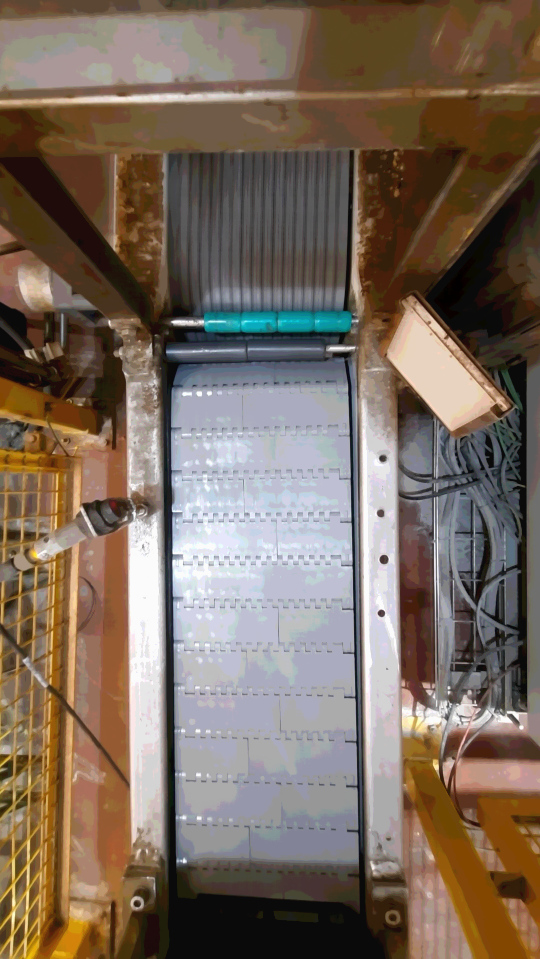
\includegraphics[width=\textwidth]{img/F1}
    \caption{Fondo Vid00.}
    \label{fig:fondo-Vid00}
\end{subfigure}
\hfill
\begin{subfigure}{0.3\textwidth}
    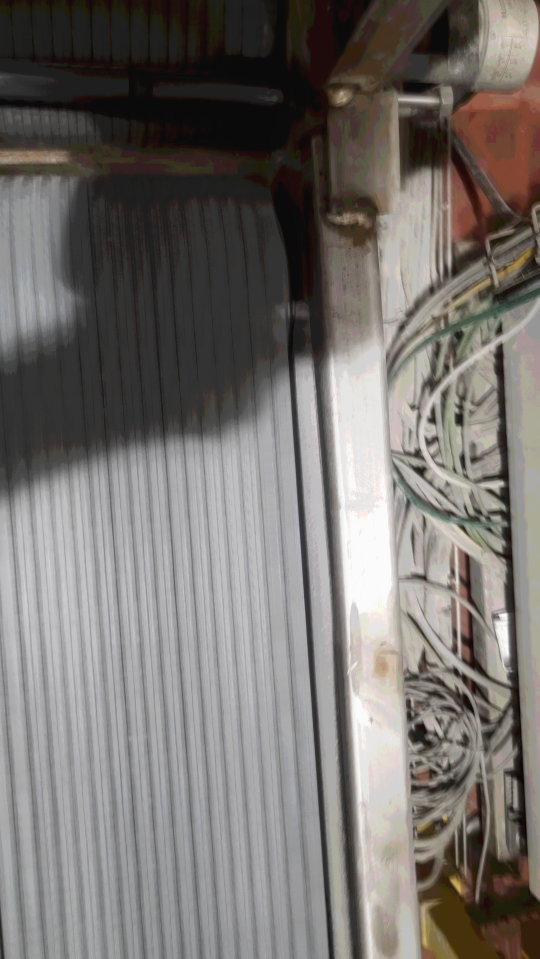
\includegraphics[width=\textwidth]{img/F2}
    \caption{Fondo Vid01.}
    \label{fig:fondo-Vid01}
\end{subfigure}
\hfill
\begin{subfigure}{0.3\textwidth}
    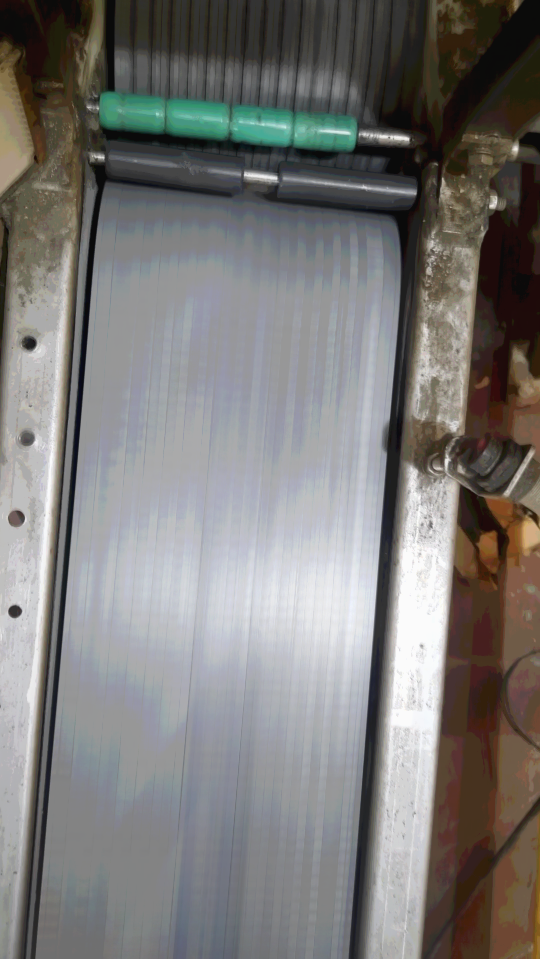
\includegraphics[width=\textwidth]{img/F3}
    \caption{Fondo Vid02}
    \label{fig:fondo-Vid02}
\end{subfigure}
\end{figure}
\end{center}

Cada \textit{frame} sufre un proceso morfológico para poder detectar los objetos que hay en él. Para ello se siguen los siguientes pasos:
\begin{enumerate}
\item Convertir el \textit{frame} a escala de grises.
\item Se resta el frame en escala de grises con el fondo general previamente calculado y pasado a escala de grises.
\item Como no trabajamos con una distancia a la cinta de transporte fija, se trabaja únicamente con un ancho de [250:750] píxeles, no con el \textit{frame} completo. Esta modificación ayuda a la detección de objetos y eliminación de ruido cuando la cámara se encuentra lejos de la cinta, y cuando estamos cerca no sufre efecto contradictorio alguno.
\item Se convierte en imagen binaria en función de un valor umbral calculado para cada \textit{frame}.
\item Se erosiona el \textit{frame} mediante <<discos>> de 12 píxeles de tamaño.
\item Se rellenan los <<huecos>> del \textit{frame}.
\item Se dilata el \textit{frame} mediante <<cuadrados>> de 80 píxeles de tamaño.
\item Se realiza un filtrado medio del \textit{frame} en dos dimensiones. Cada píxel de salida contiene el valor mediano en una vecindad de 3 por 3 alrededor del píxel correspondiente en la imagen de entrada.
\item Se elminan todos aquellos componentes conectados (objetos) que tienen menos de 200.000 píxeles, recordamos que trabajamos con una resolución de 1080x1920.
\item Detectamos los objetos restantes en la imagen.
\item Si hay objetos detectados y se encuentran dentro del área de detección y suma, área reservada donde se cuentan las baterías, éste área es la mitad inferior de la imagen, ver Figura~\ref{fig:procesado1}; se realizan cálculos para saber si es la misma batería que en el \textit{frame} anterior o no.
\item Cuando finalizan todos los \textit{frames} se obtiene una salida con el número de baterías pasadas, ver Figura~\ref{fig:salida1}.
\end{enumerate} 

Se adjuntan dos ficheros, $source.m$ y $source\_testing.m$, la diferencia sustancial es la visualización en <<tiempo real>> del procesado. En $source\_testing.m$ podemos ver la Figura~\ref{fig:procesado1}, en la cual tenemos 7 columnas. Cada una de las columnas hace representa un paso del proceso anterior, de izquierda a derecha:
\begin{enumerate}
\item Imagen resultante de la resta del \textit{frame} con el fondo, después de haber sido pasadas a escala de grises y acotadas.
\item Imagen binaria resultante.
\item Imagen resultante al proceso de erosión.
\item Imagen resultante después del rellenar los <<huecos>>.
\item Imagen resultante después de dilatar.
\item Imagen resultante después de pasar el filtro de media.
\item Imagen sobre la que buscamos los objetos después de eliminar los objetos pequeños.
\end{enumerate}

Se puede comprobar como el paso 6 es muy similar al 5, según el reflejo de las pegatinas de la propia batería, hay determinados momentos en cuales produce una pequeña diferencia, simplemente está puesto para hacer un pequeño ajuste de píxeles rebeldes, la máscara de 3x3 es muy pequeña como para alterar la imagen significativamente.

\begin{center}
\begin{figure}
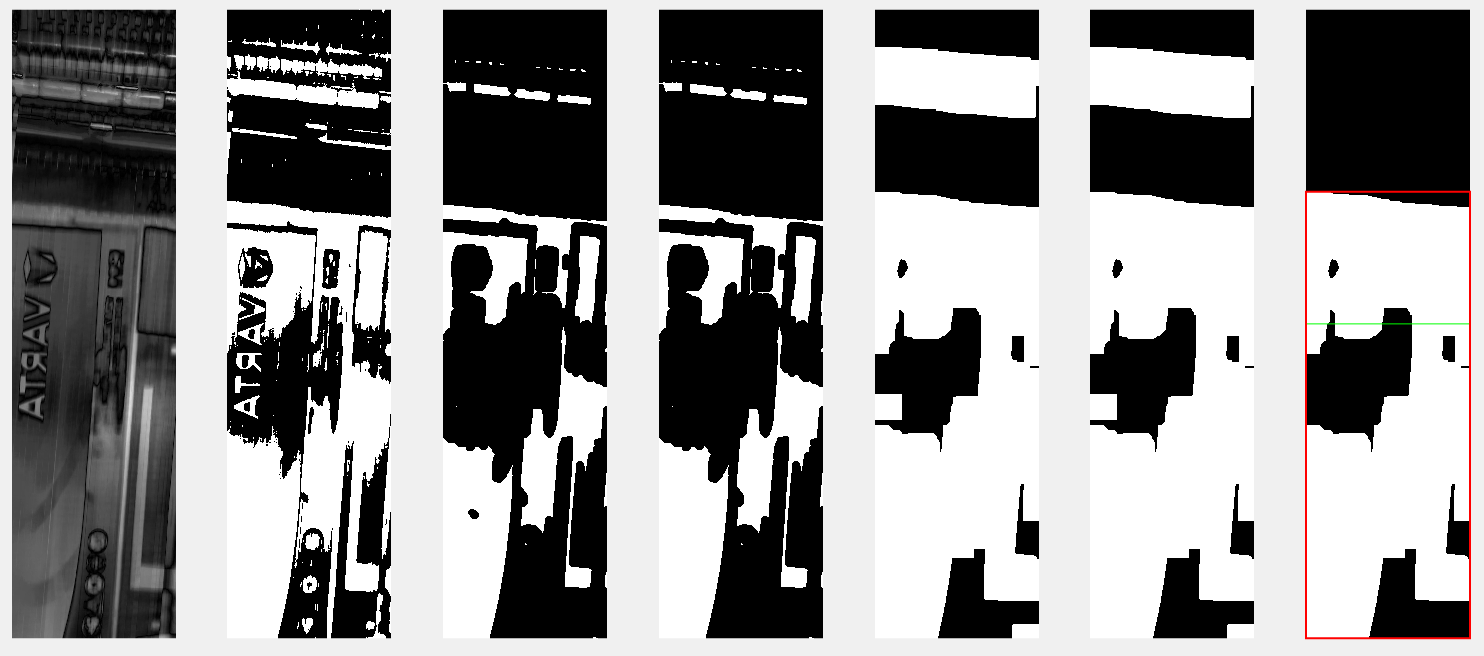
\includegraphics[width=\textwidth]{img/T1}
\caption{Procesado batería con tapa azul.}\label{fig:procesado1}
\end{figure}
\end{center}

\begin{center}
\begin{figure}
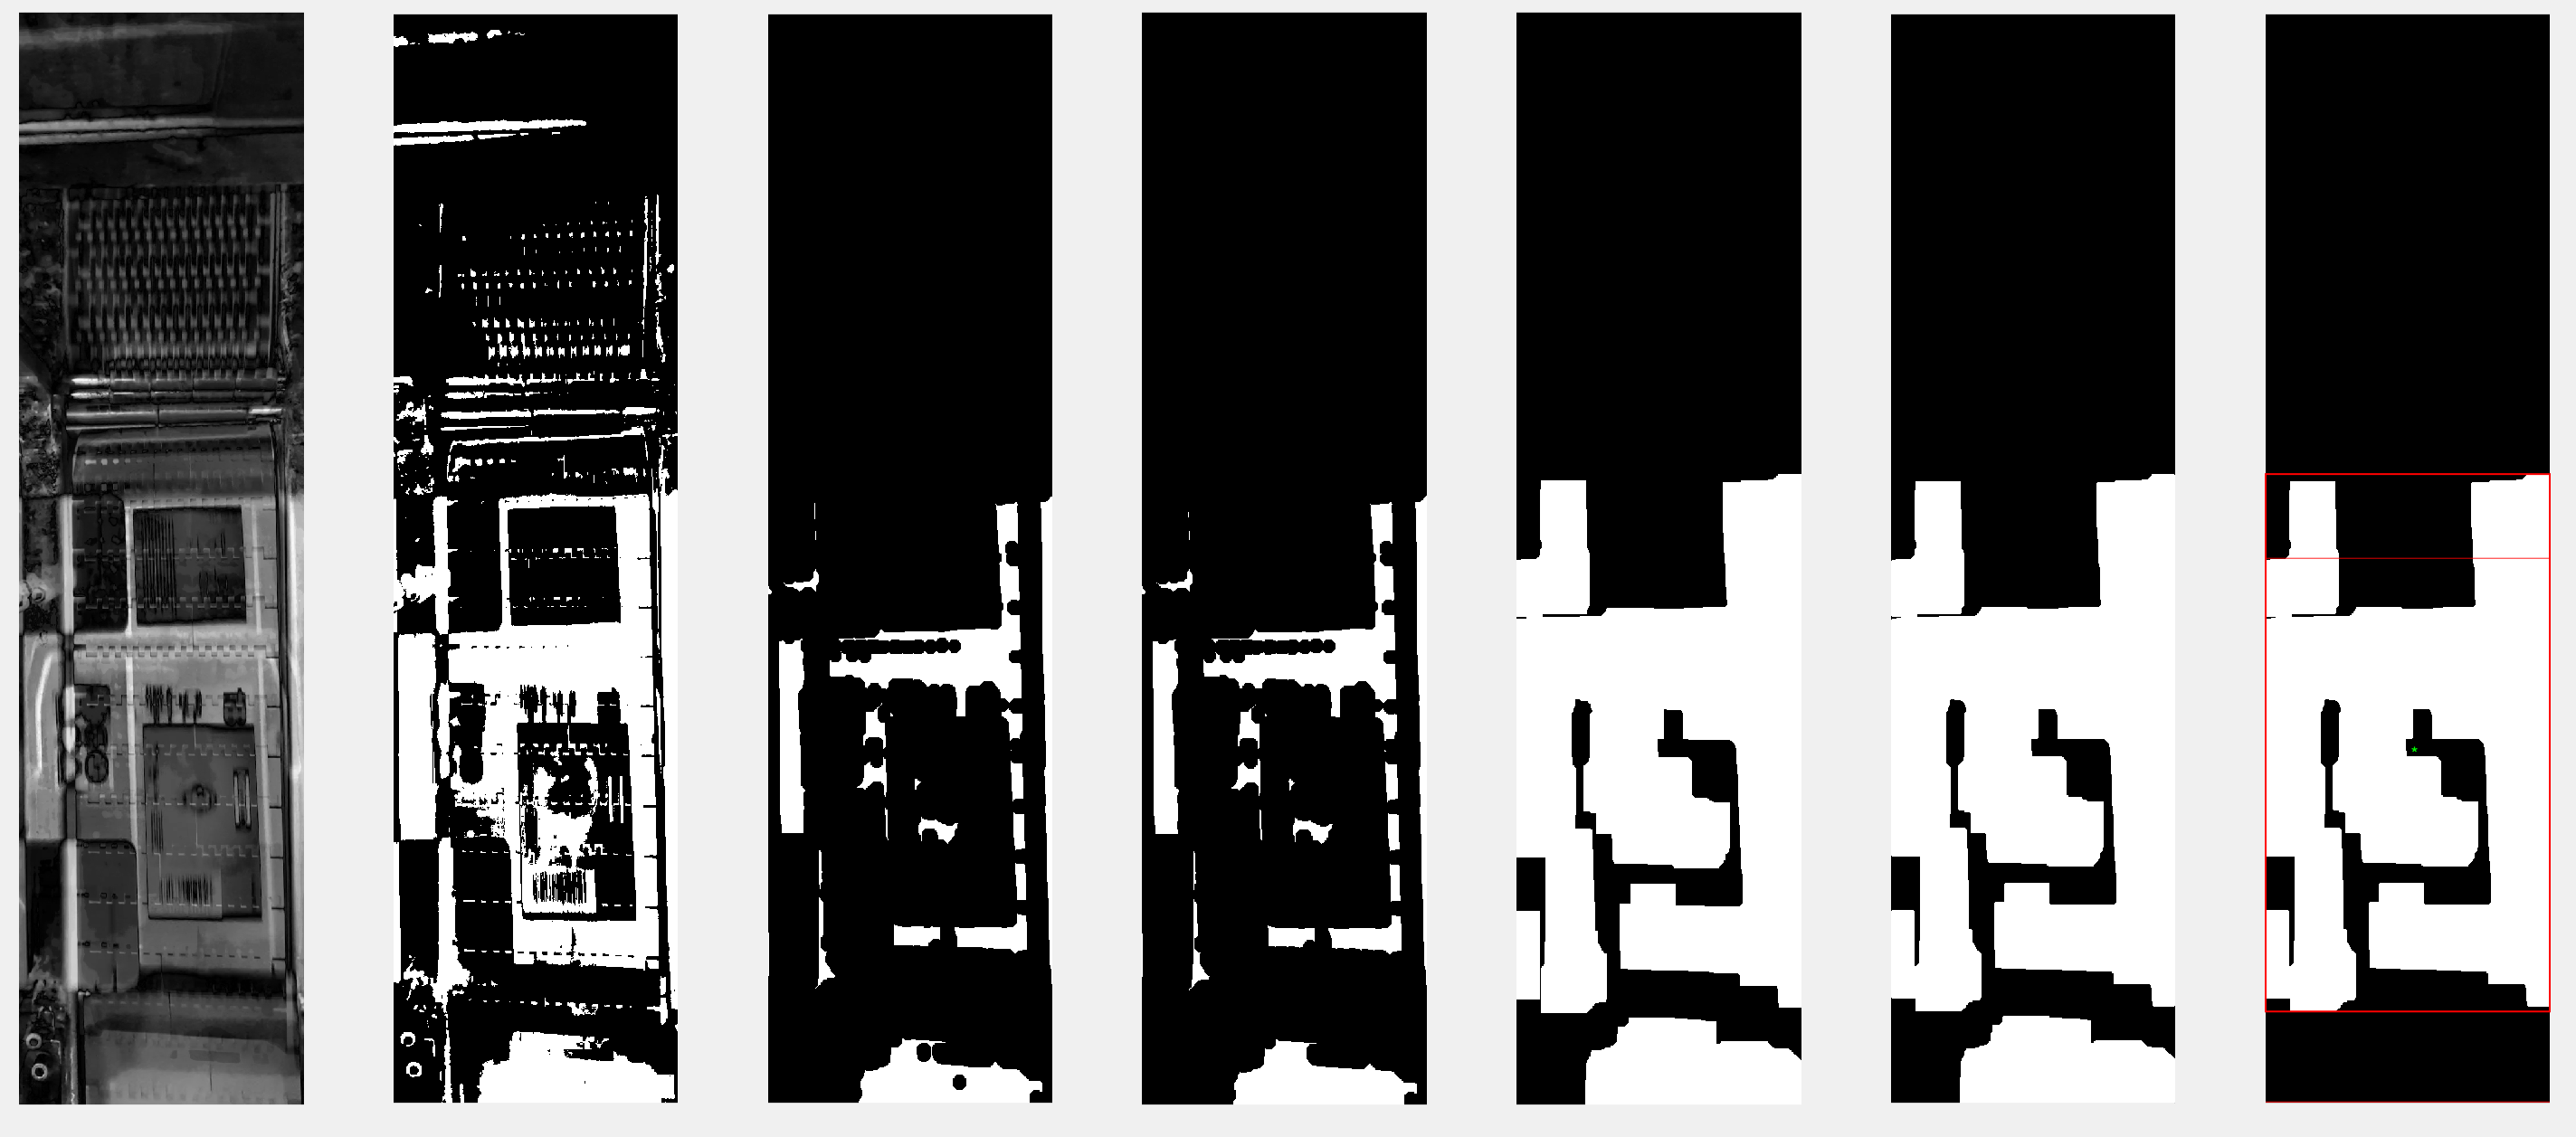
\includegraphics[width=\textwidth]{img/T3}
\caption{Procesado batería con tapa azul.}\label{fig:procesado3}
\end{figure}
\end{center}

Sobre la imagen número 7 podemos ver dos líneas verdes, una en el medio de la imagen y otra en el límite inferior, simbolizan el área de detección. Cuando el centroide del objeto detectado se encuentra dentro de ese área es cuando se cuenta la batería. Si en el \textit{frame} anteriormente analizado ya había una batería el sistema entiende que es la misma, si no la había, la computa como una nueva. Con esto da soporte a que una batería se quede parada en el área de detección, lo cual ocurre en los vídeos de prueba Vid01 y Vid02. Debido a que el avance de la cinta de transporte es mejor a 3km/h, no hay opción a que entre dos \textit{frames} salga y entre una batería, imposibilitando la no detección de una batería. En este caso esta figura está actuando sobre el Vid02, a parte del ángulo de la cinta con respecto a la cámara, la ta tapa de batería es azul y está relativamente cerca de la misma.

En la Figura~\ref{fig:procesado3} se aprecia como en el momento de la detección las líneas del área de detección cambian de color a rojo. Esta figura es resultante del Vid00, en este caso estamos más alejados de la cinta de transporte y no tenemos <<de lleno>> la intersección con la máquina anterior (parte de arriba) y una sombra considerable en la parte inferior, después de todo el procesado se es capaz de contabilizar la batería.

Sobre el fichero listo para desplegar en producción (haciendo los ajustes de vídeo para tiempo real), \textit{source.m}, nos proporciona un procesado en tiempo real de todo el \textit{frame} con sus correspondientes objetos detectados, ver Figura~\ref{fig:treal1} y~\ref{fig:treal2}.

\begin{center}
\begin{figure}[H]
\begin{subfigure}{0.4\textwidth}
    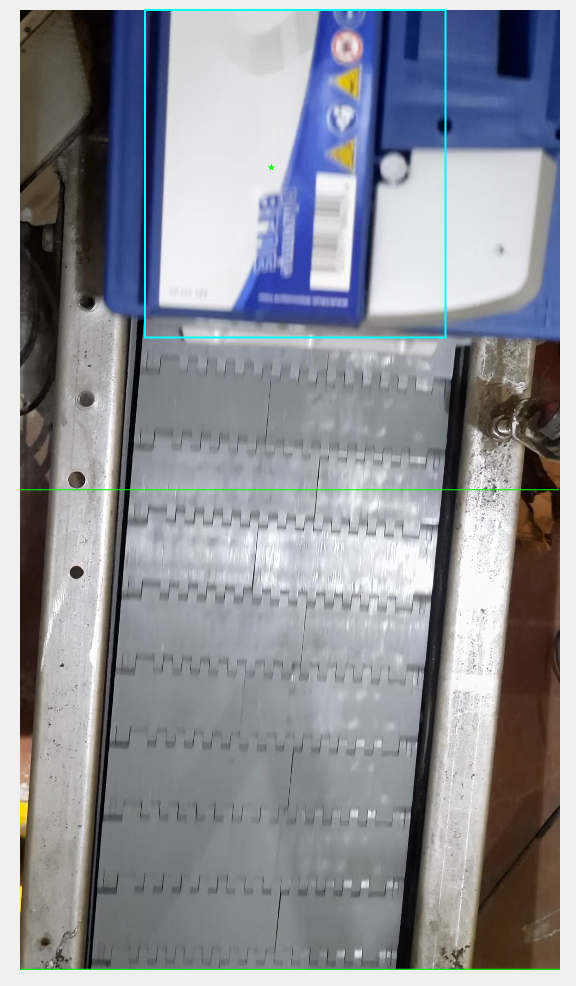
\includegraphics[width=\textwidth]{img/P1}
    \caption{Detección antes de llegar a la franja.}
    \label{fig:treal1}
\end{subfigure}
\hfill
\begin{subfigure}{0.4\textwidth}
    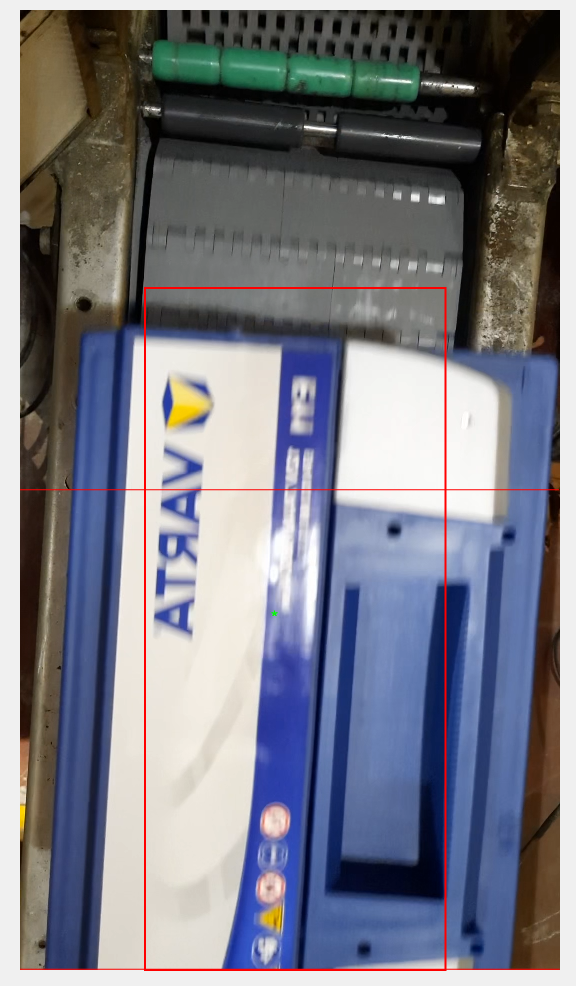
\includegraphics[width=\textwidth]{img/P2}
    \caption{Detección en la franja.}
    \label{fig:treal2}
\end{subfigure}
\end{figure}
\end{center}

\vfill
\subsection{Salida por pantalla}
La salida por pantalla que obtenemos es un \textit{pop-up} con el número de baterías que han sido contabilizadas.

\begin{center}
\begin{figure}[H]
\begin{subfigure}{0.3\textwidth}
    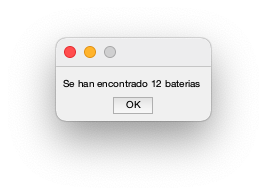
\includegraphics[width=\textwidth]{img/S0}
    \caption{12 baterías detectadas en el Vid00}
    \label{fig:salida1}
\end{subfigure}
\hfill
\begin{subfigure}{0.3\textwidth}
    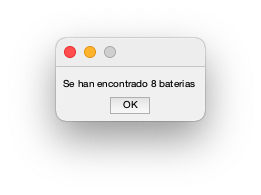
\includegraphics[width=\textwidth]{img/S1}
    \caption{8 baterías detectadas en el Vid01}
    \label{fig:salida2}
\end{subfigure}
\hfill
\begin{subfigure}{0.3\textwidth}
    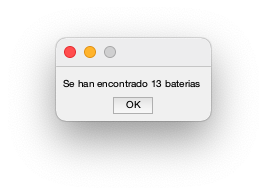
\includegraphics[width=\textwidth]{img/S2}
    \caption{13 baterías detectadas en el Vid02}
    \label{fig:salida3}
\end{subfigure}
\end{figure}
\end{center}

Finalmente podemos comprobar como son correctos los cálculos automáticos que ha hecho el \textit{software}.

\section{Opinión personal y trabajos futuros}
Si bien este software podría ser interesante para la aplicación real, tal y como está planteado. No es necesario, puesto que es el propio robot de paletizado el que se encarga de <<contar>> cuántas baterías lleva paletizadas y por ende, cuántas han pasado. 

Cuando plantee esta práctica no sabía cuántos conocimientos o técnicas vistas a lo largo del curso iban a ser consideradas, a mediados de noviembre ya con el material preparado comencé con el trabajo, antes de conocer que las últimas prácticas de la asignatura, así como el reto iban a tener una influencia tan importante en la aproximación a utilizar.

Si bien no se emplean técnicas como mapas de color, o \textit{chroma-key} o similares, no son técnicas necesarias para este proyecto.
\vfill
\begin{center}
\begin{figure}[H]
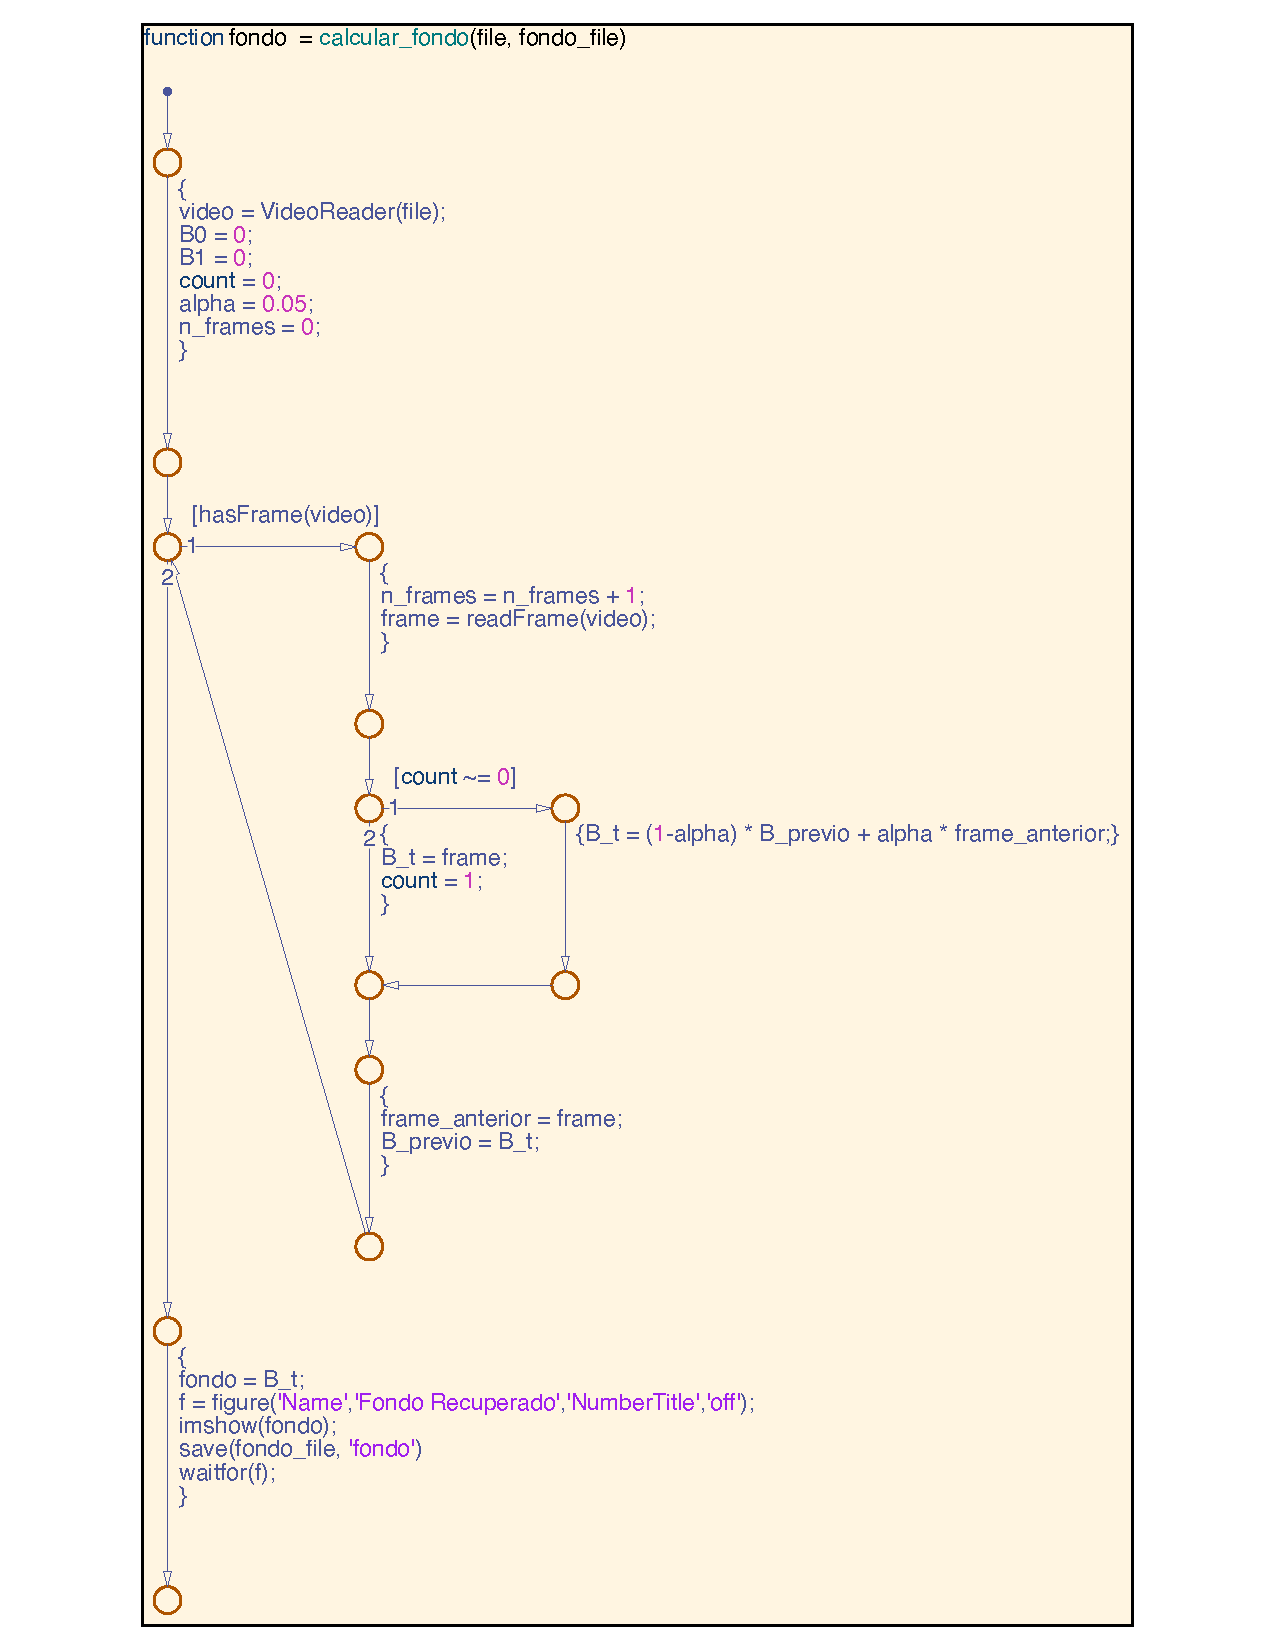
\includegraphics[width=\textwidth]{img/calc_fondo.pdf}
\caption{\textit{Stateflow} de la función que calcula el fondo de un vídeo dado.}\label{fig:calc-fondo}
\end{figure}
\end{center}
\newpage
\begin{figure}[H]
\centering
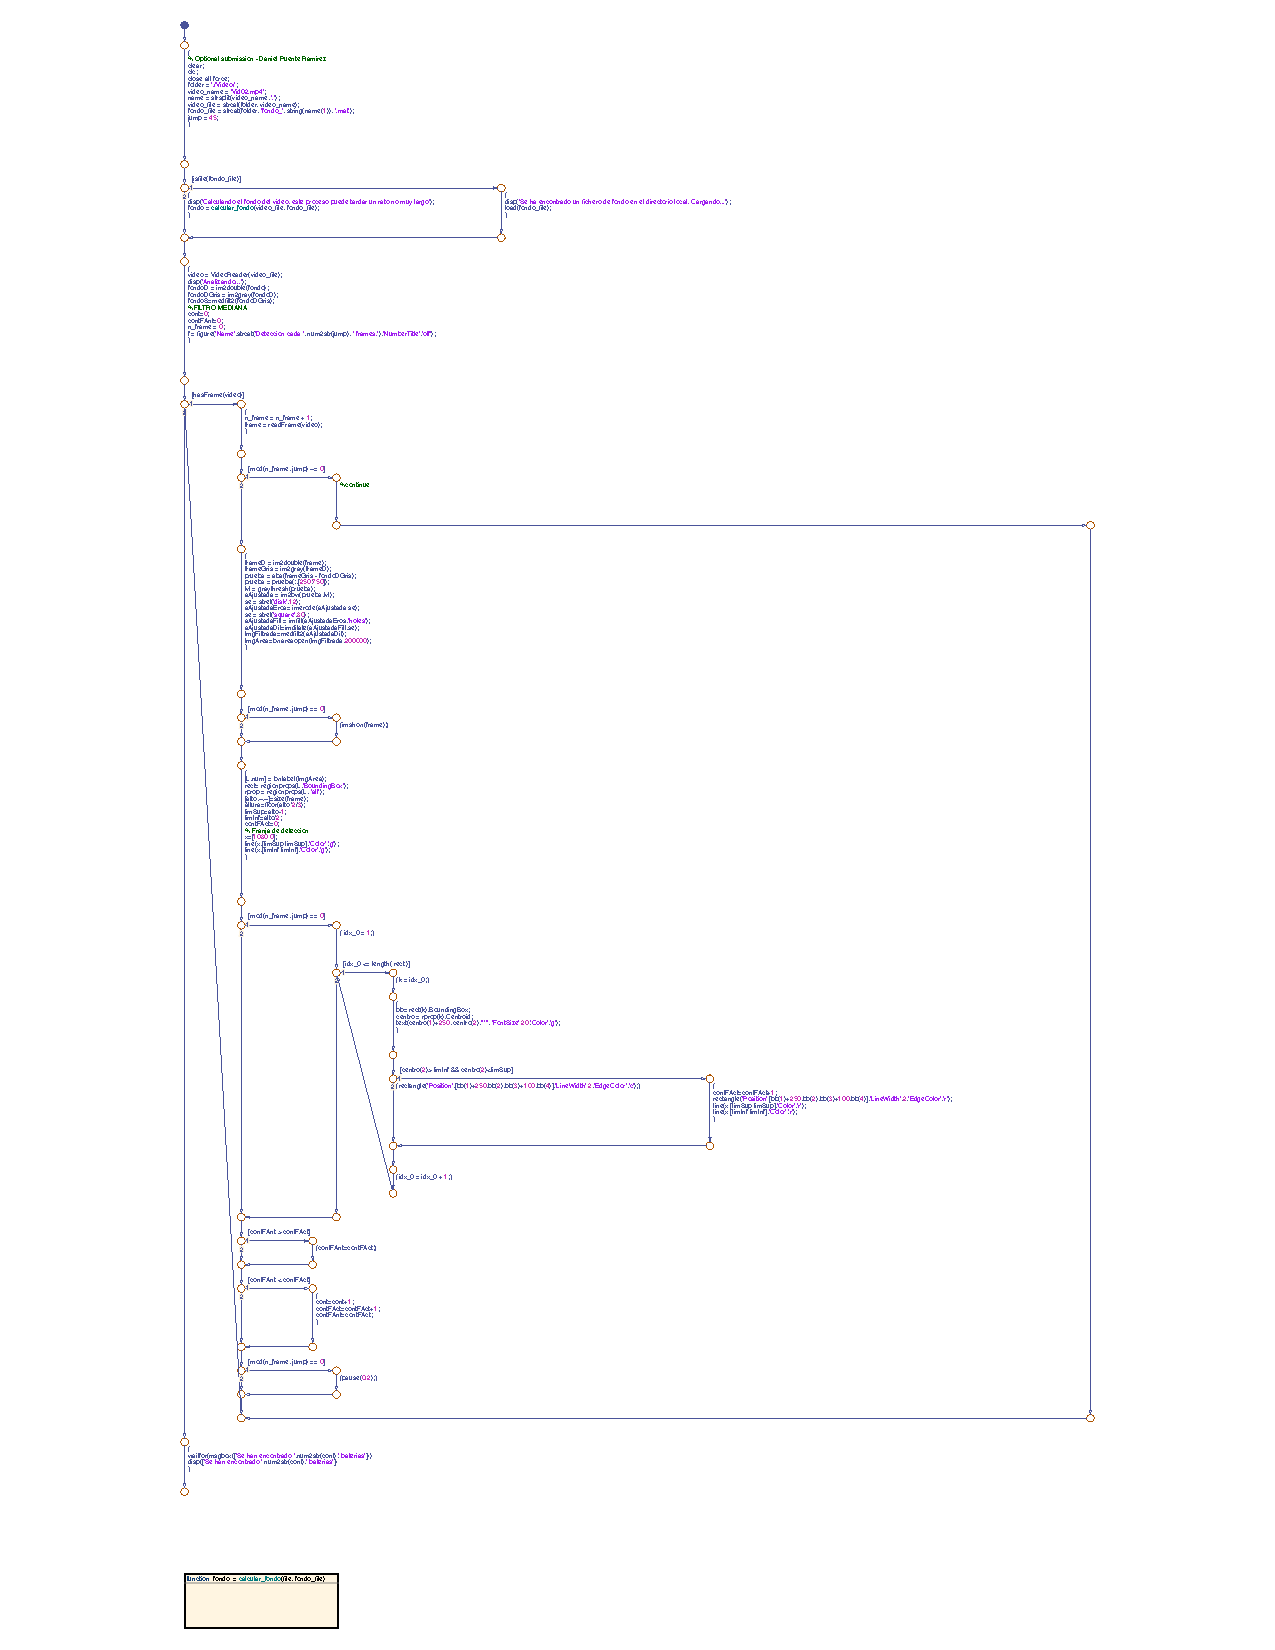
\includegraphics[scale=0.8]{img/source.pdf}
\caption{\textit{Stateflow} del código completo}\label{fig:codigo}
\end{figure}
   

\newpage
\section{Código}

\begin{lstlisting}
% Optional submission - Daniel Puente Ramirez
clear;clc;close all force;
folder = './Video/';
video_name = 'Vid02.mp4';
name = strsplit(video_name, '.');
video_file = strcat(folder, video_name);
fondo_file = strcat(folder, 'fondo_', string(name(1)), '.mat');

jump = 45;

if isfile(fondo_file)
    disp('Se ha encontrado un fichero de fondo en el directorio local. Cargando...');
    load(fondo_file);
else
    disp('Calculando el fondo del video, este proceso puede tardar un rato no muy largo');
    fondo = calcular_fondo(video_file, fondo_file);
end


video = VideoReader(video_file);
disp('Analizando...');
fondoD = im2double(fondo);
fondoDGris = im2gray(fondoD);
fondoS=medfilt2(fondoDGris); %FILTRO MEDIANA
cont=0;
contFAnt=0;


n_frame = 0;
f = figure('Name',strcat('Deteccion cada ', num2str(jump), ' frames.'),'NumberTitle','off');
while hasFrame(video)
    n_frame = n_frame + 1;
    frame = readFrame(video);
    if mod(n_frame, jump) ~= 0
        continue
    end
    frameD = im2double(frame);
    frameGris = im2gray(frameD);
    prueba = abs(frameGris - fondoDGris);
    prueba = prueba(:,[250:750]);
    
    lvl = graythresh(prueba);
    aAjustada = im2bw(prueba,lvl);
    se = strel('disk',12);
    aAjustadaEros= imerode(aAjustada,se);
    
    se = strel('square',80);
    aAjustadaFill = imfill(aAjustadaEros,'holes');
    aAjustadaDil=imdilate(aAjustadaFill,se);
    
    ImgFiltrada=medfilt2(aAjustadaDil);
    
    ImgArea=bwareaopen(ImgFiltrada,200000);
    if mod(n_frame, jump) == 0
        imshow(frame);
    end
    [L,num] = bwlabel(ImgArea);
    rect= regionprops(L,'BoundingBox');
    rprop = regionprops(L, 'all');
    
    [alto,~,~]=size(frame);
    altura=floor(alto*2/3);
    
    limSup=alto-1;
    limInf=alto/2;
    contFAct=0;
    
    % Franja de deteccion
    x=[1080 0];
    line(x,[limSup limSup],'Color','g');
    line(x,[limInf limInf],'Color','g');
    if mod(n_frame, jump) == 0
        for k=1: length(rect)
            bb= rect(k).BoundingBox;
            
            centro = rprop(k).Centroid;
            text(centro(1)+250, centro(2),"*", 'FontSize',20,'Color','g');
            
            if centro(2)> limInf && centro(2)<limSup
                contFAct=contFAct+1;
                rectangle('Position',[bb(1)+250,bb(2),bb(3)+100,bb(4)],'LineWidth',2,'EdgeColor','r');
                line(x,[limSup limSup],'Color','r');
                line(x,[limInf limInf],'Color','r');
            else
                rectangle('Position',[bb(1)+250,bb(2),bb(3)+100,bb(4)],'LineWidth',2,'EdgeColor','c');
            end
            
        end
    end
    if contFAnt > contFAct
        contFAnt=contFAct;
    end
    if contFAnt < contFAct
        cont=cont+1;
        contFAct=contFAct+1;
        contFAnt=contFAct;
    end
    
    if mod(n_frame, jump) == 0
        pause(0.2);
    end
end

waitfor(msgbox(['Se han encontrado ',num2str(cont),' baterias']))
disp(['Se han encontrado ',num2str(cont),' baterias'])


function fondo = calcular_fondo(file, fondo_file)

video = VideoReader(file);

B0 = 0;
B1 = 0;
count = 0;
alpha = 0.05;
n_frames = 0;
while hasFrame(video)
    n_frames = n_frames + 1;
    frame = readFrame(video);
    if count ~= 0
        B_t = (1-alpha) * B_previo + alpha * frame_anterior;
    else
        B_t = frame;
        count = 1;
    end
    frame_anterior = frame;
    B_previo = B_t;
end
fondo = B_t;
f = figure('Name','Fondo Recuperado','NumberTitle','off');
imshow(fondo);
save(fondo_file, 'fondo')
waitfor(f);
end
\end{lstlisting}

\section{Material utilizado}
A continuación se dejan enlaces a todo el material utilizado, para uso en futuros trabajos, independientemente de si son de la universidad, proyectos públicos o privados, se ha de consultar al autor del documento.

\begin{itemize}
\item Vídeos utilizados.
\begin{itemize}
\item \href{https://universidaddeburgos-my.sharepoint.com/:v:/g/personal/dpr1005_alu_ubu_es/EblH-8CwOBxFveSSffVrCSIBAsXnm-RjX1KjU1Q9CDcHGw?e=4ioTBW}{Vid00}
\item \href{https://universidaddeburgos-my.sharepoint.com/:v:/g/personal/dpr1005_alu_ubu_es/EbD-vo49t31ItwpNTlBO92EBx-xBuX7tSuepVe4B4PEW_Q?e=58hLev}{Vid01}
\item \href{https://universidaddeburgos-my.sharepoint.com/:v:/g/personal/dpr1005_alu_ubu_es/EWApw-KIdKdNvyhZXxp9HywBpRJ9XWvZNaMFYzPMy5yTpA?e=sH9AGl}{Vid02}
\end{itemize}
\item \href{https://github.com/dpr1005/Car-battery-detection-system}{Repositorio de Github}
\begin{itemize}
\item \href{https://github.com/dpr1005/Car-battery-detection-system/blob/master/source.m}{\textit{source.m}}
\item \href{https://github.com/dpr1005/Car-battery-detection-system/blob/master/source_testing.m}{\textit{source-testing.m}}
\end{itemize}
\end{itemize}
\vspace{2cm}


\clearpage
\thispagestyle{empty}
\vspace*{\fill}
\begin{center}
\begin{figure}[b]
\begin{subfigure}{0.4\textwidth}
    
\includegraphics[height=2cm]{img/Escudo}
\end{subfigure}
\hfill
\begin{subfigure}{0.4\textwidth}
    
\includegraphics[width=\textwidth]{img/Clarios}
\end{subfigure}
\end{figure}
\end{center}

Copyright \textcopyright\ 2021 Daniel Puente Ramírez All rights reserved.


    

\end{document}